%%%%%%%%%%%%%%%%%%%%%%%%%%%%%%%%%%%%%%%%%%%%%%%%%%%%%%%%%%%%%%%%%%%%%%%
%                          template.tex
%
% LaTeX template for papers conforming to the United States Sections of
% the Combustion Institute style guide.
%
% Authors:
%     Bryan W. Weber, University of Connecticut
%     Kyle E. Niemeyer, Oregon State University
%
% This work is licensed under the Creative Commons Attribution 4.0
% International License. To view a copy of this license, visit
% http://creativecommons.org/licenses/by/4.0/.
%
% The source for this template can be found at
% https://github.com/pr-omethe-us/ussci-latex-template
%%%%%%%%%%%%%%%%%%%%%%%%%%%%%%%%%%%%%%%%%%%%%%%%%%%%%%%%%%%%%%%%%%%%%%%
\documentclass[12pt]{ussci}

%======================================================================
% Remove this in the real document
\usepackage{adjustbox}
\usepackage{amsmath}
\usepackage{amsfonts}   % if you want the fonts
\usepackage{amssymb}    % if you want extra symbols
\usepackage{booktabs}
\usepackage{bm}
\usepackage{chemformula}
\usepackage{float}
%\usepackage{fourier}
\usepackage{footnote}
\usepackage{multirow}
\usepackage[hang,flushmargin,bottom]{footmisc} % footnote format

\usepackage{graphicx}   % need for figures
\usepackage{mathptmx}
\usepackage{multicol}
\usepackage{physics}
\usepackage{rotating}
\usepackage{secdot}
\usepackage{siunitx} % Formats the units and values
\usepackage{tabulary}
\usepackage{textgreek}
\usepackage{textcomp}
\usepackage{tikz}
\usepackage[flushleft]{threeparttable}
\usepackage[utf8]{inputenc}
\usepackage[T1]{fontenc}
\usepackage{xcolor}
\usepackage{footmisc}
\usepackage[english]{babel}
%\usepackage(biber}
%%\usepackage[backend=biber,
%style=alphabetic,
%citestyle=authoryear
%]{biblatex}
%======================================================================
% BibLaTeX and biber (not BibTeX) are used to process the references,
% so these packages must be installed on your system. All configuration
% for the bibliography and citations are done in the ussci.cls file
% Add your bibliography file here, replacing template.bib
\addbibresource{USCIM_Propane_Pool_Fires.bib}
%======================================================================
% Replace "Reaction Kinetics" in the line below by your paper topic
\newcommand\papertopic{Fire Research}
%======================================================================

\title{The structure of medium-scale propane pool fires}

\author[*1]{Ryan Falkenstein-Smith}
\author{Kunhyuk Sung}
\author{Anthony Hamins}

\affil[1]{National Institute of Standards and Technology, Gaithersburg, MD, USA}
\affil[*]{Corresponding author: \email{ryan.falkenstein-smith@nist.gov}}

\begin{document}
\maketitle

%====================================================================
\begin{abstract} % not to exceed 200 words
A series of time-averaged temperature, velocity, and gas species measurements are made along the centerline of propane fires established on a 37~cm diameter gas burner situated in a quiescent environment.  Fires with heat release rates of 20 kW and 34 kW are selected for study to complement previous measurements of total heat flux emitted to the surroundings in these fires. Gas samples are extracted at various heights above the burner centerline and analyzed using a Gas Chromatograph with mass selectivity and thermal conductivity detectors. Soot mass fractions are gravimetrically measured. Major gas species, including propane, oxygen, carbon dioxide, water, carbon monoxide, hydrogen, nitrogen, argon, and soot, are detected and quantified. Intermediate gas species are observed to achieve peak concentrations a few cm above the fuel surface, whereas carbon dioxide and water peak further downstream. The chemical and physical structures of the fires are compared by considering the profiles of measured gas species volume fractions, soot mass fractions, temperature and velocity profiles.  Plotting the temperature and velocity profiles as a function of z* collapse the experimental data and provide insight into the structure of these medium-scale propane pool fires.
\end{abstract}

% Provide 2-4 keywords describing your research. Only abbreviations firmly
% established in the field may be used. These keywords will be used for
% sessioning/indexing purposes. Use \sep between each keyword.
\begin{keyword}
 Gas pool fires\sep Gas species measurements\sep Propane flame structure
\end{keyword}

%====================================================================
\section{Introduction}
%
Computation fluid dynamics fire models are an important component to performance based design in fire protection engineering. A requirement of their acceptance and prominent usage are verifying and validating the developed models, the latter of which involves comparison with experimental measurements. This objective of this work is to provide measurements for validation in fire model validation. 

Pool fires are a convenient test bed for model validation due to their flat, horizontal, and isothermal fuel surface which provides a well-defined boundary-condition for modeling. A zone of particular interest is the fue-rich core between the flame and pool surface, where gas species can absorb energy that would otherwise have been transferred to the fuel surface. Therefore, gas species concentrations, temperature, and velocity measurements are of interest. However, few studies in literature have reported local chemical species measurements within the flame~\cite{Fisher1987,Hamins2016,Choi1995,andrews2005,meier2000,bundy2007,Lock2008,Falkenstein2021a,Falkenstein2020a,Falkenstein2020b,Falkenstein2021b,ORLOFF1988General,ORLOFF1987Chemical,smith1992major}. 

The purpose of this study is to characterize the spatial distribution of the temperature, velocity, and principal chemical species in medium-scale propane pool fire steadily burning in a well ventilated, quiescent environment. Propane is selected as the fuel of interest, burned at different fire sizes. A series of fire experiments are conducted using a 37~cm effective diameter pool burner. Gaseous species, soot, temperature, and velocity measurement are made at various locations with the centerline of the propane fires. The measurement techniques applied in this study are justified based on previous work in fire literature~\cite{Falkenstein2021c,Choi1995}.


\section{Methods/Experimental}
\subsection{Pool Burner Setup}
All experiments are conducted under a canopy hood surrounded by four 2.5~m x 2.5~m wire-mesh screen (5~ mesh/cm), which reduces the impact of room ventilation. All measurements are made once the mass rate of the fire reaches steady-state, achieved approximately 2~min after ignition. 
The propane fires are burned using a round 37~cm effective diameter, porous metal burner. The gas burner is maintained at a constant temperature by circulating cooled water (approximately \SI{20}{\degree C} $\pm$ \SI{5}{\degree C}. Fuel to the gas burner is controlled via a Brooks mass flow controller, Model 5863\footnote{\label{fn:product} Certain commercial products are identified in this report to specify adequately the equipment used. Such identification does not imply a recommendation by the National Institute of Standards and Technology, nor does it imply that this equipment is the best available for the purpose.} located outside the enclosure. Description of previous pool fires experiments are found in Refs.~\cite{Hamins2016,Hamins1994,Hamins1991,Hamins1996a,Hamins1996b,Lock2008}

The mean flame height is estimated from 3600 frames of high-resolution video of the steady-state propane pool fires using MATLAB's Image Processing Toolbox. The flame height of a single frame is defined by the distance between the pool surface and observed flame tip. All measurements are repeated, then averaged to provide the mean flame height. 

\subsection{Temperature Measurements}\label{ssec:Temp_Meas}
Time-averaged temperature measurements are made at varying positions along the centerline profiles of the pool fires. A S-type (Pt, 10\% Rh/Pt), bare-wire, thermocouple (OMEGA P10R-001) with a 50~$\mu$m wire diameter and a bead diameter approximately 150~$\mu$m is used. Temperature measurements are sampled at nominally 250~Hz for 2~min, or approximately 300 pulsing cycles~\cite{Falkenstein2021a}. Optical microscope observations show that the thermocouple bead is spherical. 

To account for the unsteady flow field, thermocouple temperature measurements are corrected for heat losses and thermal inertia following Shaddix~\cite{Shaddix2001}, in which conduction losses are assumed to be small and the compensation for thermal inertia is calculated from the Nusselt number via the Ranz-Marshall model~\cite{Shaddix1999}. The temperature-dependent gas properties for the Reynolds and Prandtl numbers are taken as those of air from Ref.~\cite{Incropera2011}.  The temperature-dependent emmissivity and thermophysical properties of platinum are taken from Refs.~\cite{Platinum2010, Jaeger1939}. A detailed description of the measurement and its uncertainty is described in Refs.~\cite{Sung2020}. 

\subsection{Velocity Measurements}
Time-averaged velocity measurements are made using a bi-directional probe positioned about the burner's centerline. A full description of the measurement and its uncertainty is provided in Ref.~\cite{Sung2021}. The instantaneous gas velocity is determined from the pressure difference between the front and rear of the probe. The differential pressure is measured with multiple pressure transducers, with varying instrument response times, sampling between 250 to 500~Hz for a period of 2~min. Temperature-dependent gas properties are taken as those of air and are calculated using temperature measurements made 5~mm below the probe. Temperature measurements are made using the same method described in Section~\ref{ssec:Temp_Meas}. 

\subsection{Volume Fraction of Gas Species Measurements}
Time-averaged gas species volume fraction, $\bar{X}_{i}$, measurements are made using an Agilent 5977E Series Gas Chromatograph with thermal conductivity and mass selectivity detectors (GC/MSD). Gas samples are extracted using a thermal quenching prove composed of concentric, stainless-steel tubes with an outer annular coolant flow and inner extracted sample flow. The quenching probe's temperate is maintained by a heated water reservoir (approximately \SI{90}{\degree C}) which flow through the probe for the duration of the experiment. Directly behind the quenching probe is a heated sampling line, heated to approximately \SI{140}{\degree C}) to prevent water from condensing within the line. The heated sampling line also includes a soot filter, used to provide time-average soot measurements, and a 150~ml mixing chamber, that ensures the sample is well-mixed and is an accurate representation of the local volume of interest.

The gas sampling flow rate is controlled via a mass flow controller located between the GC/MSD and vacuum pump. During the gas sampling procedure, the volumetric flow is approximately 200~mL/min and recorded at 2~Hz. Gas sampling time is dependent on the probe location withing the fire, with the sampling period varying from 12 to 25~min. All gas species measurements at a given location are repeated at least twice.The mean mass fraction, $\bar{Y}_{i}$, of a given species $i$ is calculated from the measured volume fraction using the following expression:
\begin{equation}\label{eq:mass_fraction}
	\bar{Y}_{i}=\frac{\bar{X}_{i} \, {\textrm{W}_{i}}}{\sum{\bar{X}_{i} \, {\textrm{W}_{i}}}}
\end{equation}
where ${{\textrm{W}_{i}}}$ is the molecular weight of a given species. A detailed description of the gas species measurement and its uncertainty is documented in several other works~\cite{Falkenstein2021a}. 

\subsection{Soot Mass Fraction Measurements}
Soot mass fraction, $Y_{\rm s}$, is measured using a well established gravimetric technique. Soot is filter out from the extracted gas sample directly behind the thermal quenching probe. Before sampling a desiccated 47~mm polytetrafluoroethylene (PTFE) filter is weighed and placed into a stainless steel particulate filter holder (PALL 2220). After sampling, the PTFE filter is removed and dried in a desiccator for 48~h where in after the filter weight is measured. 
After most experiments, soot deposits are observed on the inner walls of the quenching probe and are extracted using desiccated gun cleaning patches (Hoppe's 9 1203S). At least two patch are used to collect soot on the inside of the probe. Soot collection on the inside of the probe concludes once an applied patch is observed to have no soot. Similar to PTFE filters, patches are weighed immediately before and 48~h after extraction. 
The soot mass fraction is  from the determined from mass of the soot collected from the PTFE filter and gun cleaning patches, $m_{\rm s}$, the ratio of the downstream temperature measured at the mass flow controller and time-averaged temperature measurements described in Section~\ref{ssec:Temp_Meas}, and the total mass of gas sampled, $m_{\rm tot}$.
\begin{equation}\label{eq:soot_mass_frac}
Y_{s}= \frac{m_{\rm s}}{m_{\rm tot}}
\end{equation}
The total mass of gas sampled is the product of the average volumetric flow rate measured by the mass flow controller, $\dot{V}$, the density of the sample gas injected into the GC/ms, $\rho_{\rm gas}$, the gas sampling time, $\Delta t$. 
\begin{equation}\label{eq:total_mass}
m_{t}= \dot{V} \, \rho_{gas}\, \Delta t \frac{T_{\infty}}{T_{\rm g}}
\end{equation}

A description of the soot mass fraction measurement and uncertainty is provided in greater detail in Ref.~\cite{ Falkenstein2021a}. 

\subsection{Uncertainty Analysis}
An extensive uncertainty analysis of all measurements is provided in Refs.~\cite{Sung2020,Sung2021, Falkenstein2021a}. Measurement uncertainties are estimated using the law of propagation of uncertainty which combines the Type A and B evaluation of uncertainty. For most measurements, the Type A evaluation of uncertainty is the dominant error. Unless otherwise stated, the uncertainty of the measurements are expressed assuming a 95\% confidence level. 

\section{Results and Discussion}
\subsection{Flame Observations}
The measured time-averaged burning rates and calculated heat release rates are provided in Table~\ref{tab:Pool_Fire_Parameters_Table}. The heat release rate, $\dot{Q}$, is estimated from the product of the mass burning rate, $\dot{m}$, and the heat of combustion,$\Delta H_{\rm c}$, of the fuel. The measured mean flame heights, $L_{\rm f}$, are observed to match with Heskestad's correlation, shown in Eq.~\ref{eq:Flame_height}, to within the measured uncertainty.
\begin{equation}\label{eq:Flame_height}
\frac{L_{\rm f}}{D} = 3.7 \, (\dot{Q}^*)^{2/5} - 1.02 \quad ; \quad \dot{Q}^*=\frac{\dot{Q}}{c_{p}\rho_\infty T_\infty \sqrt{g} \, D^{5/2}}
\end{equation}
Here, $D$ is the diameter of the pool fire (30~cm), $g$ is the acceleration of gravity, and $c_p$ and $\rho_\infty$ are the specific heat and the density of air at room temperature, $T_\infty$. 

\begin{table}[!t]
\caption[List of measurements and thermochemical properties of fuels]{List of measurements and thermochemical properties of propane burning in a well-ventilated round 37~cm diameter pool fire burning in a quiescent environment.}
\label{tab:Pool_Fire_Parameters_Table}
\centering
	\footnotesize
	\begin{tabular}{p{0.125\linewidth}p{0.1\linewidth}p{0.1\linewidth}p{0.1\linewidth}p{0.1\linewidth}p{0.1\linewidth}p{0.1\linewidth}}
\hline
%\\[0.0005cm]
{Fuel} &{$\dot{m}$}& { $\dot{Q}$}& {$\dot{Q}^* $}&{$D^*$}&{$L_{\rm f}$}&{$\Delta H_{\rm c}$~\cite{SFPE}}\\
{-} &{(\si{g/{s}})}& {(\si{kW})}& {}&{(\si{m})}&{(\si{cm})}&{(kJ/g)}\\
\hline
\\[0.01cm]
Propane		&	0.74~$\pm$~0.01 & 34.4~$\pm$~0.6 & 0.37~$\pm$~0.01 & 0.25~$\pm$~0.01 & 50.0~$\pm$~16.0 & 46.34\\
\\[0.01cm]
Propane		&	0.45~$\pm$~0.01 & 20.7~$\pm$~0.6 &0.22~$\pm$~0.01 & 0.20~$\pm$~0.01 &	38.3~$\pm$~14.6 & 46.34\\
\hline
\end{tabular}
\end{table}

\subsection{Comparison of Fire Structure}
To compare the propane pool fires of different sizes, the temperature, velocity, and gas species measurements are plotted as a function of the normalized vertical spatial coordinate, $z^*$:
\begin{equation}\label{eq:Z_Star}
z^*=\frac{z}{D^*}  \quad ; \quad  D^* = \left(\frac{\dot{Q}}{c_{p}\rho_\infty T_\infty \sqrt{g}}\right)^{\frac{2}{5}}
\end{equation}
Here, $z$ is the vertical spatial coordinate, $\dot{Q}$ is the heat release rate, $g$ is the acceleration of gravity, and $c_p$ and $\rho_\infty$ are the specific heat and the density of air at room temperature, $T_\infty$.

Figure~\ref{fig:Temp_Comparison} displays the time-averaged gas temperature measurements of the 20~kW and 34~kW propane fires as a function of $z^*$.  The time-averaged temperatures of the 20~kW and 34~kW propane fires are observed to peak within the flame ($z^* <$ 1.32~\cite{Baum1989}) at a $z^*$ equal to 0.56 and 0.98, respectively. The maximum time-averaged temperature for each pool fire is close to 1325~K. 
\begin{figure}[h!]
	\centering
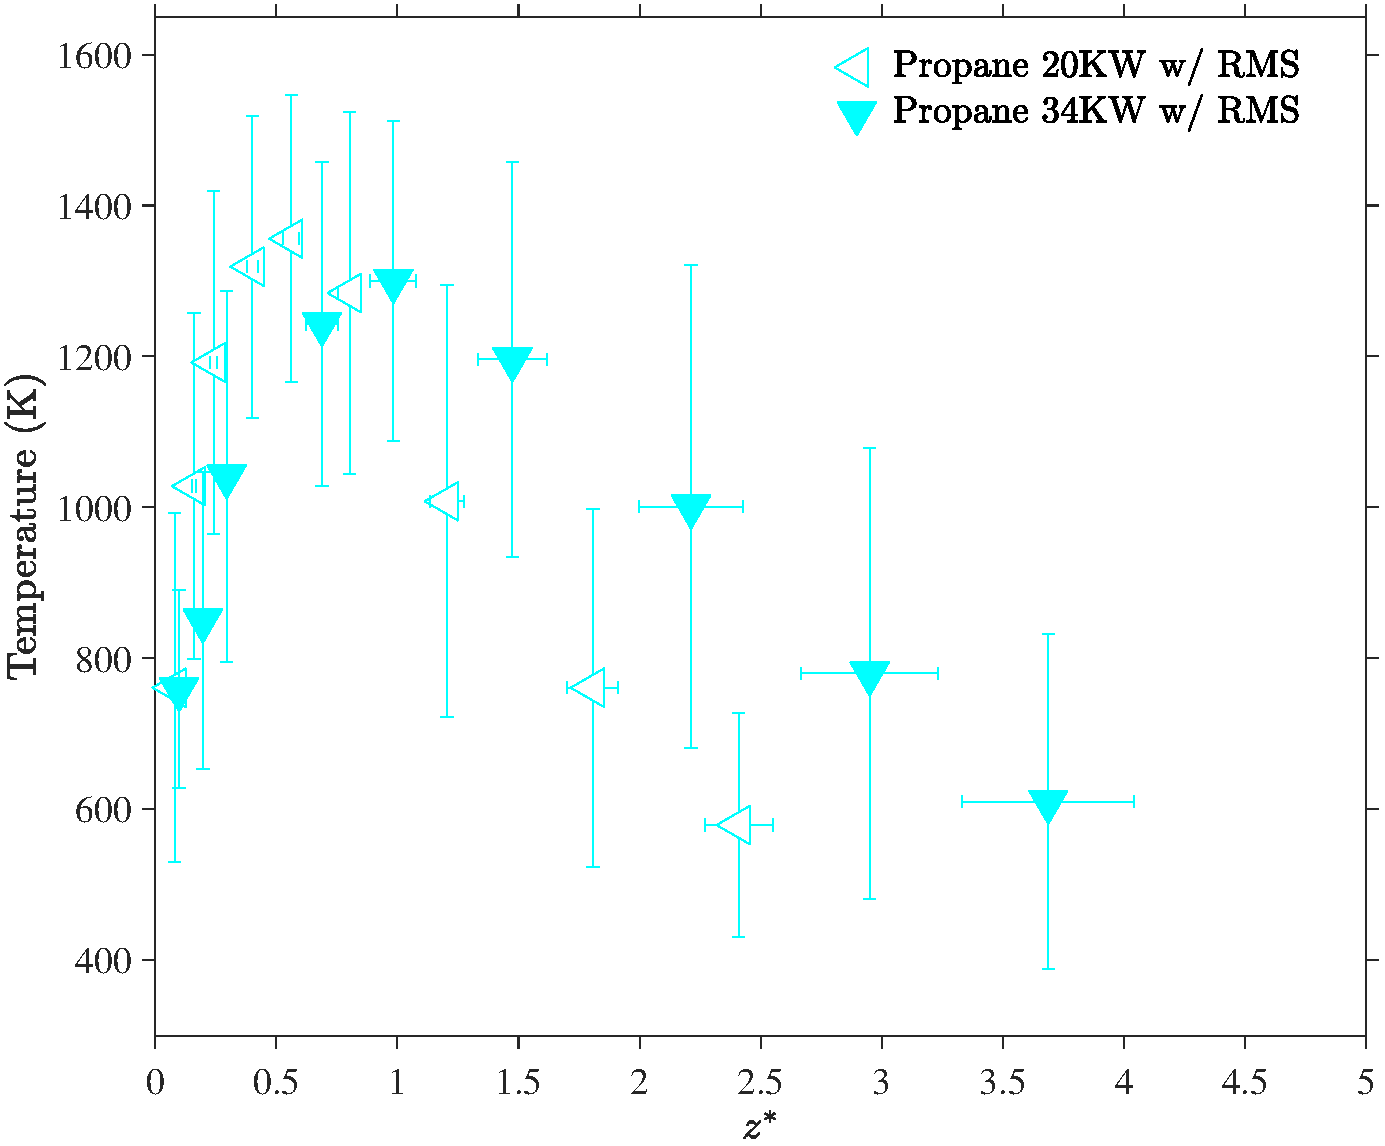
\includegraphics[width=8 cm, keepaspectratio]{Temperature.pdf}
	\caption[Mean and RMS centerline gas temperature profiles]{Mean and root mean square (RMS) centerline gas temperature profiles of propane pool fires during their pulsing cycles as a function of $z^*$.}
	\label{fig:Temp_Comparison}
\end{figure}

Time-averaged velocity measurements are presented as a function of $z^*$ in Fig.~\ref{fig:Vel_Comparison}. The velocity of the both propane fires are shown to increase within the flame, then achieve a consistent value (approx. 3.4~m/s) in the intermittent section of the fire (1.32 $< z^* <$ 3.3~\cite{Baum1989}). When plotted as a function of $z^*$, the velocity profiles of both propane fires are shown to collapse, suggesting that the flow field within the different size fires evolve in a similar manner. 
\begin{figure}[h!]
	\centering
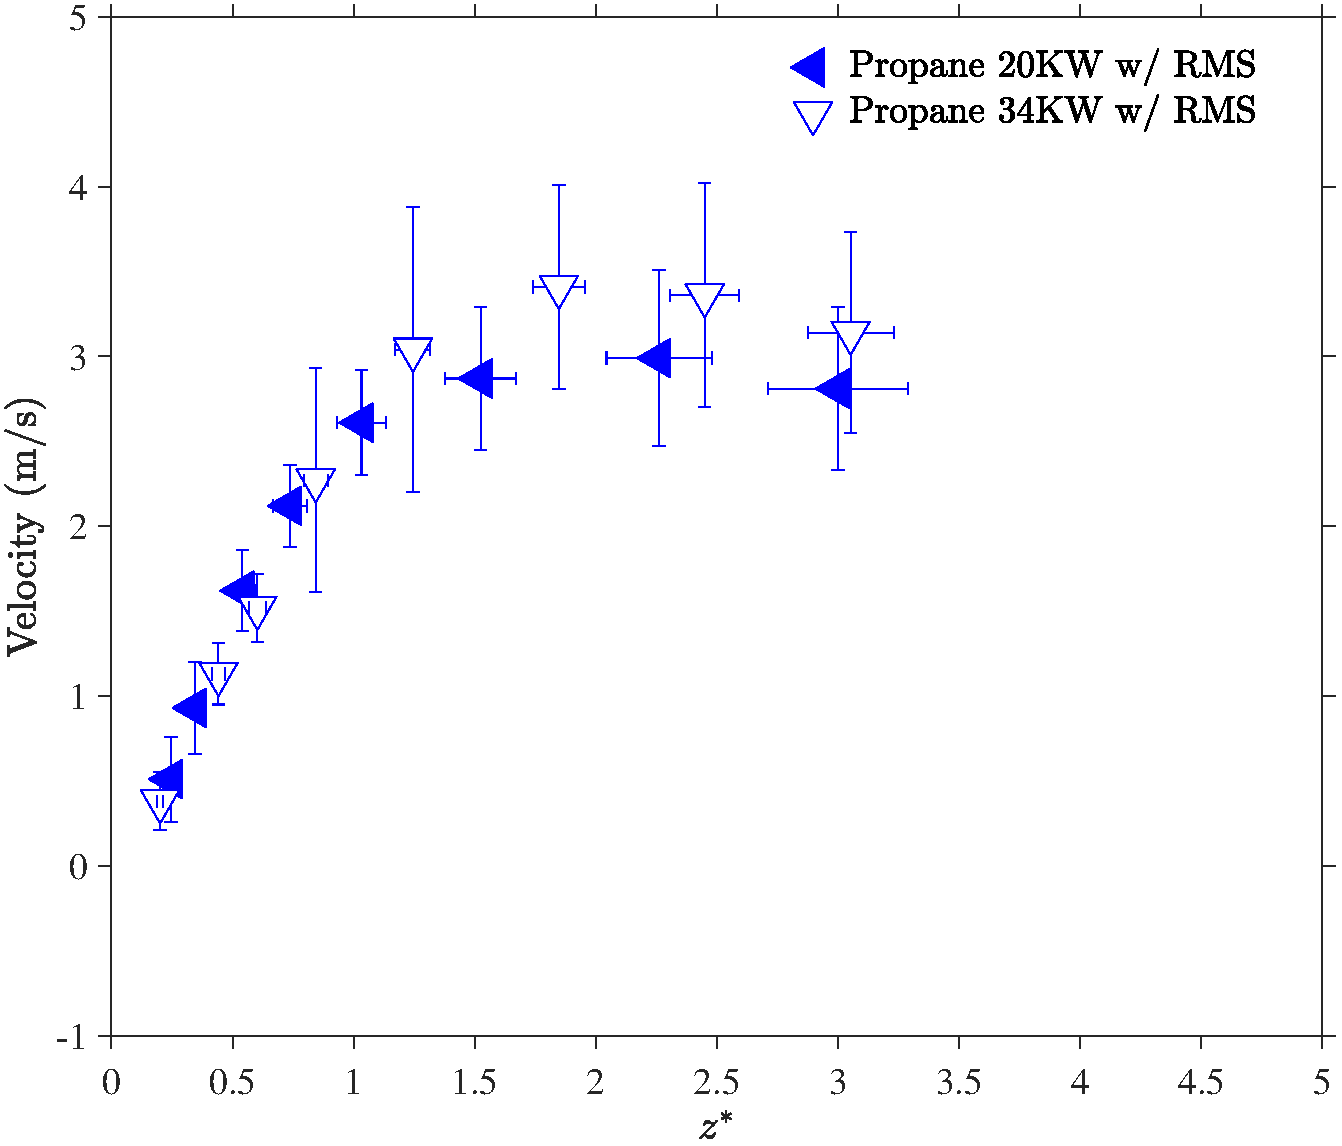
\includegraphics[width=8 cm, keepaspectratio]{Velocity.pdf}
	\caption[Mean and RMS centerline velocity profiles]{Mean and root mean square (RMS) centerline velocity profiles of and propane pool fires during their pulsing cycles as a function of $z^*$.}
	\label{fig:Vel_Comparison}
\end{figure}

The time-averaged gas volume fraction of major gas species and the mass fraction of soot for the 20~kW and 34~kW propane fires are shown in Figure~\ref{fig:Fuel_Comparison}, plotted as a function of $z^*$. Plots for individual species, including uncertainties, are reported in Ref.~\cite{Falkenstein2021a}. Major species detected in the GC/MSD include combustion reactants (propane, $\ch{C3H8}$, and oxygen, $\ch{O2}$), combustion products (carbon dioxide, $\ch{CO2}$, and water, $\ch{H2O}$), combustion intermediates (carbon monoxide, $\ch{CO}$, and hydrogen, $\ch{H2}$), and inert gases (nitrogen, $\ch{N2}$ and argon, $\ch{Ar}$). Trace concentrations of other species are also observed such as methane, ethane, ethylene, acetylene, propene, soot, and benzene. 
\begin{figure}[!]
	\centering
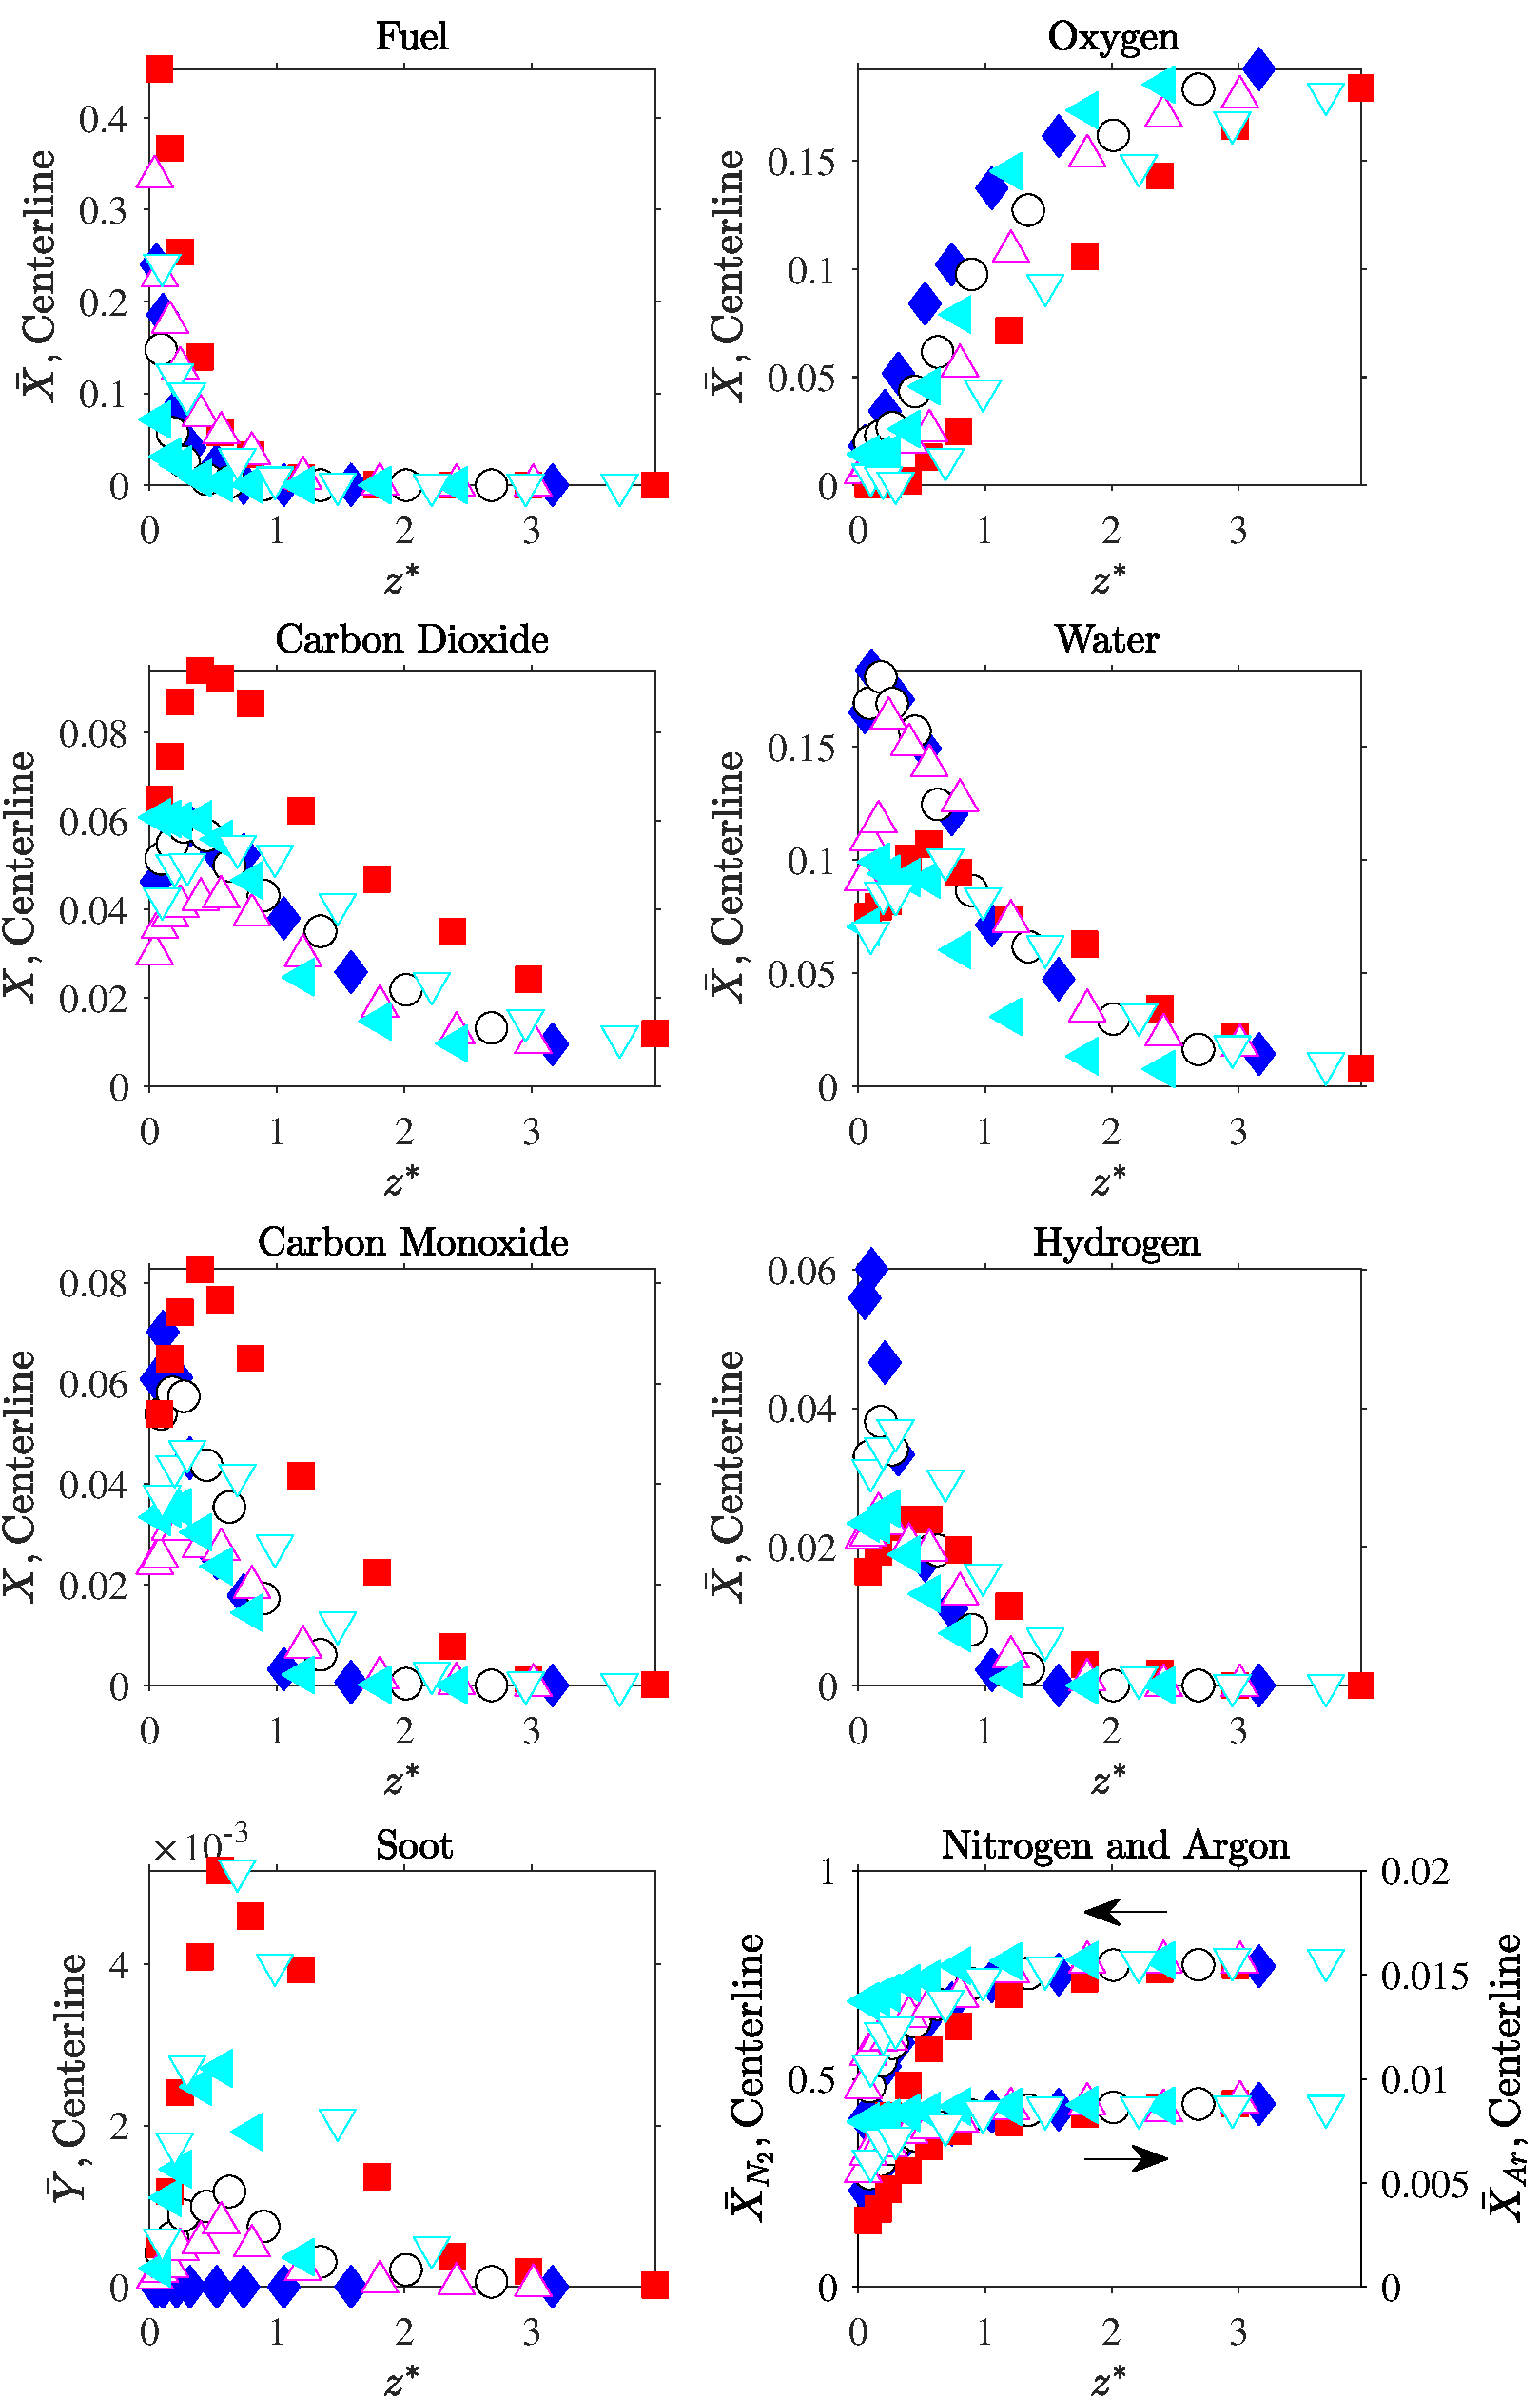
\includegraphics[width=12.5cm,keepaspectratio]{OVERALL_Fuel_Comparison.pdf}
	\caption[Centerline volume fraction and soot mass fraction profiles]{Centerline volume fraction and soot mass fraction profiles of a 20~kW propane ($\blacktriangleleft$) and 34~kW propane ($\bigtriangledown$) pool fires as a function of $z^*$.}
	\label{fig:Fuel_Comparison}
\end{figure}

For both fires, the fuel concentrations are shown to decline as the distance from the fuel surface increases, contrary to oxygen which increases. The intermittent species are observed to peak closer to the fuel surface compared to carbon dioxide and hydrogen. In comparison to the 20~kW propane fire, the 34~kW propane fire is shown to have a higher peak soot mass fraction by approximately a factor of 2. 

The carbon to hydrogen ratio is calculated, using Eq.~\ref{eq:c2h_ratio}, at each measurement location as a way to verify the accuracy of the experimental gas species concentrations measurements. 

\begin{equation}\label{eq:c2h_ratio}
  \frac{\rm C}{\rm H}= \frac{\textrm{W}_{\rm{C}}}{\textrm{W}_{\rm{H}}}\, \frac{ \sum  {\rm x}_i \, \bar{X}_{i}}{\sum {\rm y}_i \, \bar{X}_{i}}
\end{equation}
Here the summation over all measured gas species, and ${\rm x}_i$ and ${\rm y}_i$ are the numbers of carbon and hydrogen atoms in the molecule, respectively. For the case of propane, the theoretical carbon to hydrogen ratio is 0.375 and the ratio for each fuel is shown in Fig.~\ref{fig:C2H}. As seen in Fig.~\ref{fig:C2H}, the theoretical carbon-to-hydrogen ratio for propane, represented by the dotted line, is in agreement with the gaseous species measurements with the experimental uncertainty. The conservation of the carbon to hydrogen ratio at each position for each fuel validates the experimental setup and indicates that the loss of condensable or semi-volatile species during extraction is minimal. 
\begin{figure}[h!]
	\centering
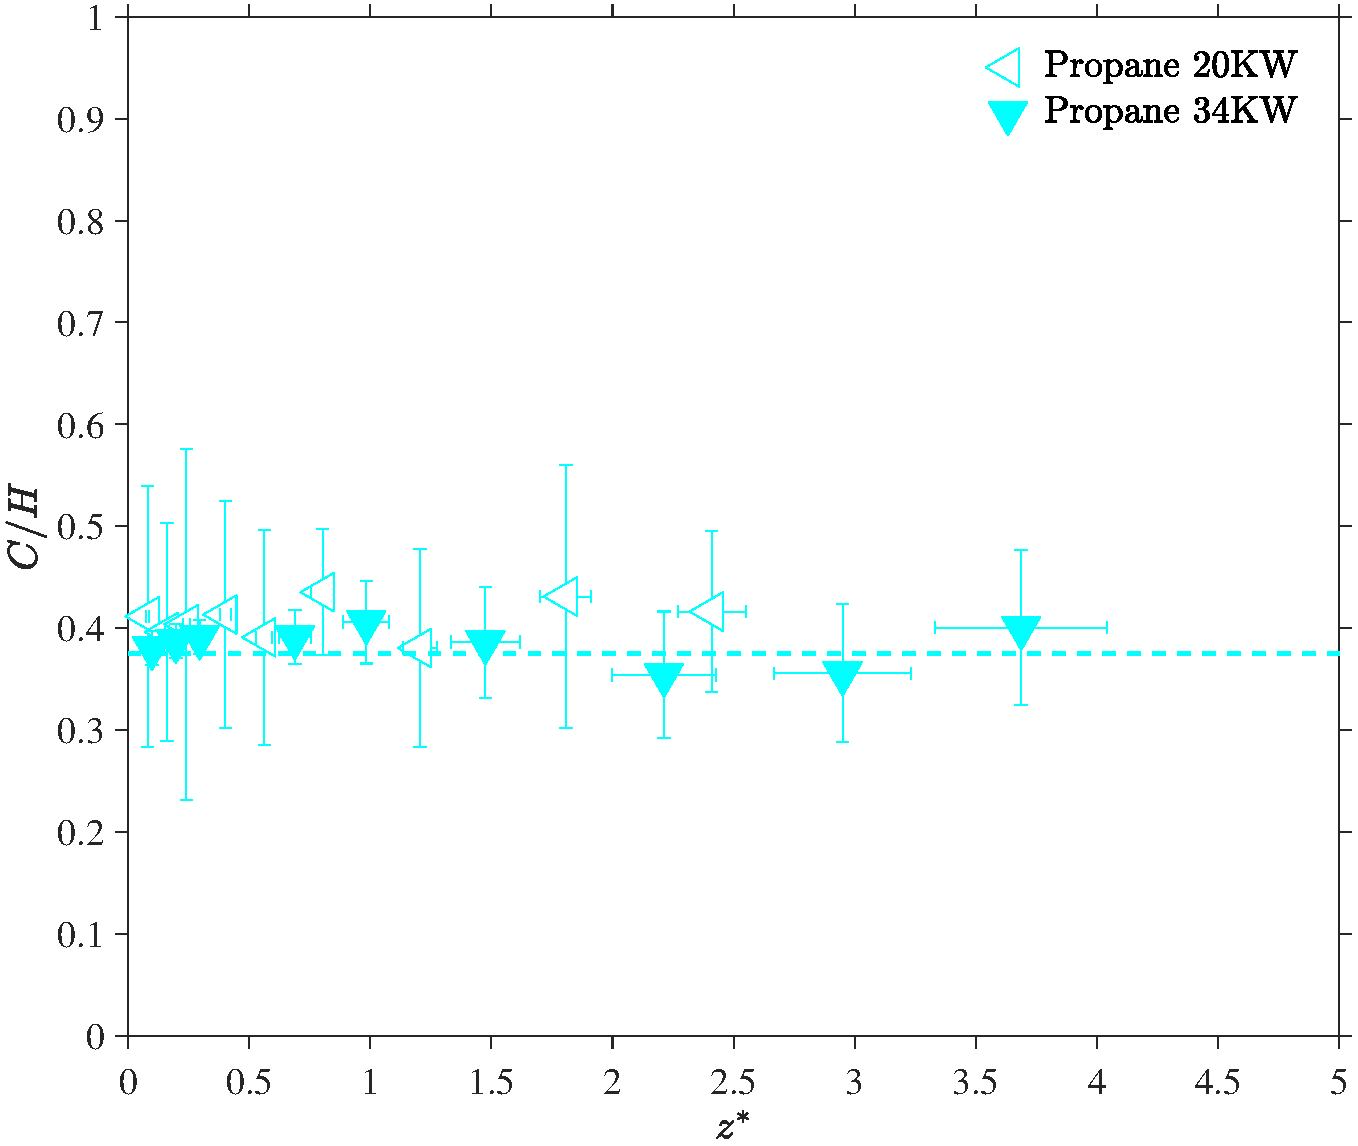
\includegraphics[width=8cm, keepaspectratio]{CtoH_Ratio.pdf}
	\caption[Carbon to hydrogen ratio calculated from all species]{Carbon to hydrogen ratio calculated from all measured gas species compared to the theoretical values as a function of $z^*$.}
	\label{fig:C2H}
\end{figure}

\subsection{Carbon Balance}
Carbon containing species measured within the propane fires were primarily partitioned into carbon dioxide, carbon monoxide, methane, and soot. Figure~\ref{fig:C2S} displays the mass ratio of carbon monoxide to soot as function of $z^*$ for both propane fires.  The general trend of each fuel shows that the ratio of carbon monoxide to soot decreases as the distance from the fuel surface increases. As observed, when plotted as a function of $z^*$, the mass ratio of carbon monoxide to soot measured from each propane fire of different size tends to collapse, suggesting that carbon is partitioned similarly within propane fires of different size. K\"{o}yl\"{u} et al.~\cite{koylu1991} reported that the mass-based ratio of $\ch{CO}$ to soot generation factors in the overfire (i.e., the fuel-lean exhaust stream) region of non-premixed hydrocarbon flames for a range of strongly sooting fuels was $0.34~\pm~0.09$. It is observed that the ratio of $\ch{CO}$ to soot tends to K\"{o}yl\"{u}'s a locations higher within fires' plume. Similar results have been previously documented. It should be noted however, that the measurements made here are primarily within the flame envelope, whereas K\"{o}yl\"{u}'s are in the overfire region~\cite{koylu1991}.
\begin{figure}[h!]
	\centering
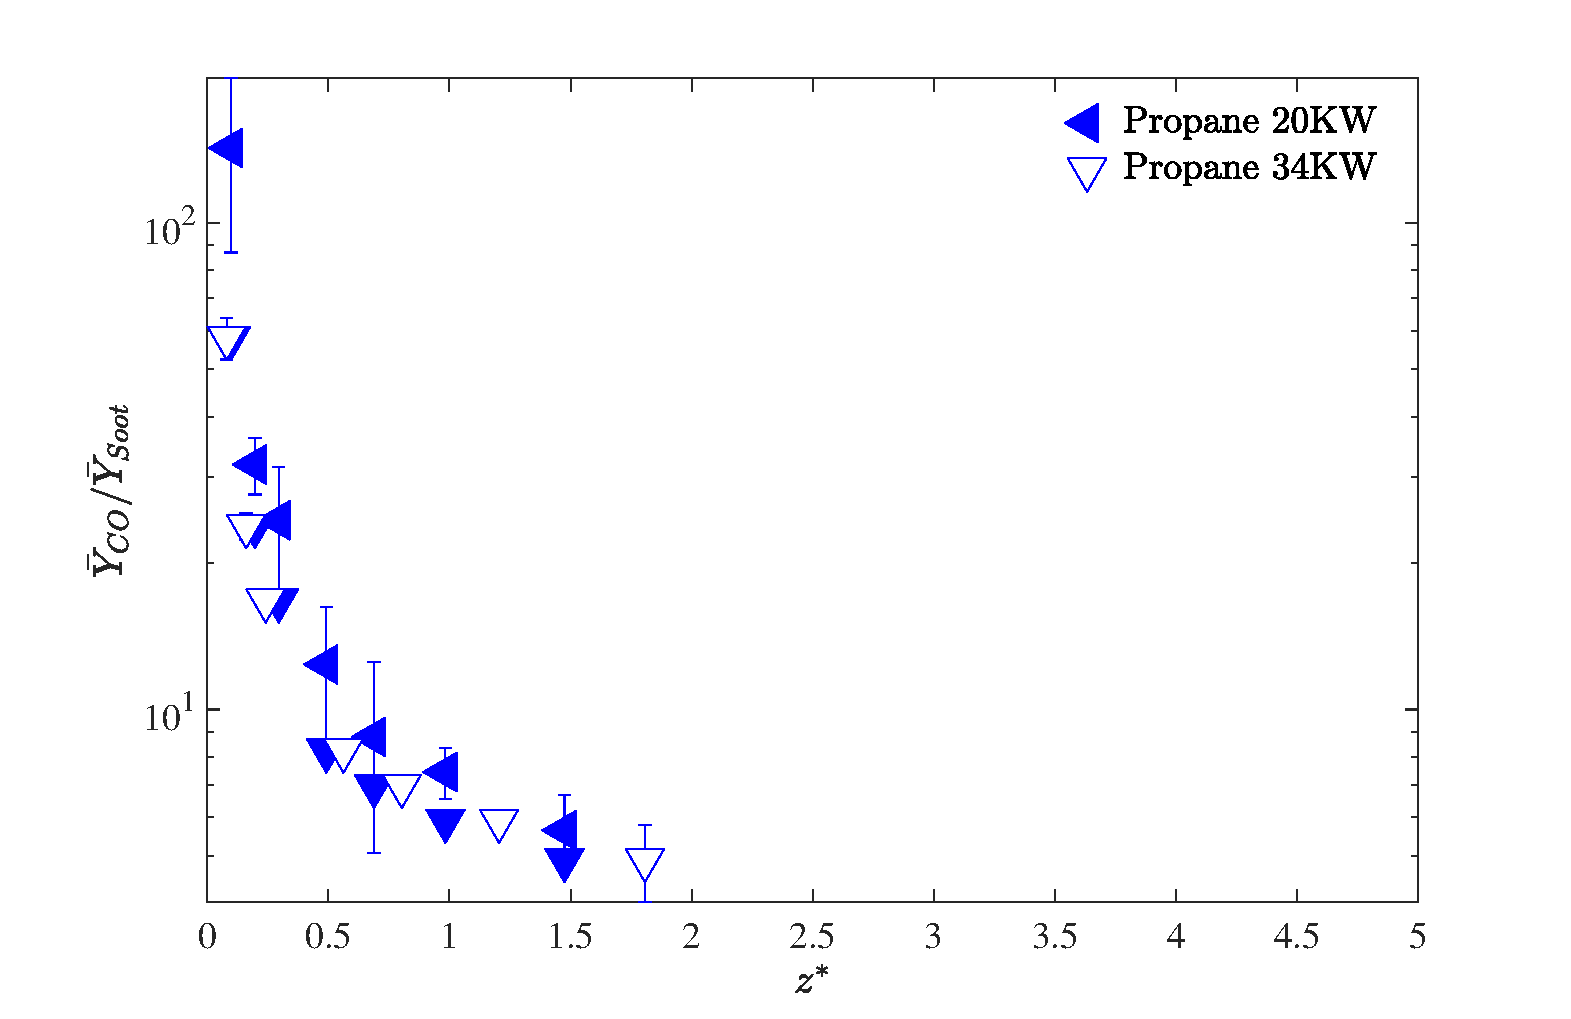
\includegraphics[width=8cm, keepaspectratio]{CO_Soot.pdf}
	\caption[Carbon monoxide to soot ratio as a function of mixture fraction]{Carbon monoxide to soot ratio as a function of $z^*$.}
	\label{fig:C2S}
\end{figure}

\section{Conclusions}
This study characterizes the structure of two medium-scale propane pool fires steadily burning in a quiescent environment. Temperature, velocity, gas species concentrations for a 20~kW and 34~kW propane fire are reported. The temperature and velocty profiles collapse when plotted as a function of $z^*$. The calculated carbon-to-hydrogen ratio is shown to be in agreement with the theoretical value at each location. As expected, as the fire heat release rate is increased, the peak concentrations on the fire centerline of soot, $\ch{CO}$, and $\ch{H2}$ in the fire significantly increase.  For a factor of 1.7 increase in the fuel flow, the peak soot, $\ch{CO}$, and $\ch{H2}$ centerline concentrations go up by a factor of 2, 1.4, and 1.9, respectively.  Robust chemistry sub-models are needed that can address these non-linear finite rate chemistry effects. Future work will apply the same technique to different size propane fires to see if observed trends are consistent. This technique will also be applied to non-centerline positions and pool fires of different fuels to further expand the repository of datasets that will help guide the development and validation of CFD fire models. . 


%\bibliographystyle{elsarticle-num.bst}
%\bibliography{template} %%User-specified

\printbibliography

\end{document}
